\documentclass[aspectratio=169]{beamer}
\setbeamertemplate{navigation symbols}{}
\usepackage{color,amsmath,comment, subfigure}
\usepackage{booktabs}
\def\vf{\vfill}
\usepackage{url}

\def\imagetop#1{\vtop{\null\hbox{#1}}} %http://tex.stackexchange.com/questions/23521/tabular-vertical-alignment-to-top

%\setbeameroption{show notes}

%%%%%%%%%%%%%%%%%%%%%%%%%%
\title[]{Class 17: Going viral}
\author[]{Matthew J. Salganik}
\institute[]{Sociology 204: Social Networks\\Princeton University}
\date[]{
1/2 What does viral look like?
\vfill

\begin{flushleft}
\vspace{0.6in}

\includegraphics[width=0.1\textwidth]{figures/cc.png}
\end{flushleft}
}

\begin{document}
%%%%%%%%%%%%%%%%%%%%%%%%%%%
\frame{\titlepage}
%%%%%%%%%%%%%%%%%%%%%%%%%%%
\begin{frame}

What does it mean to go viral?

\begin{center}
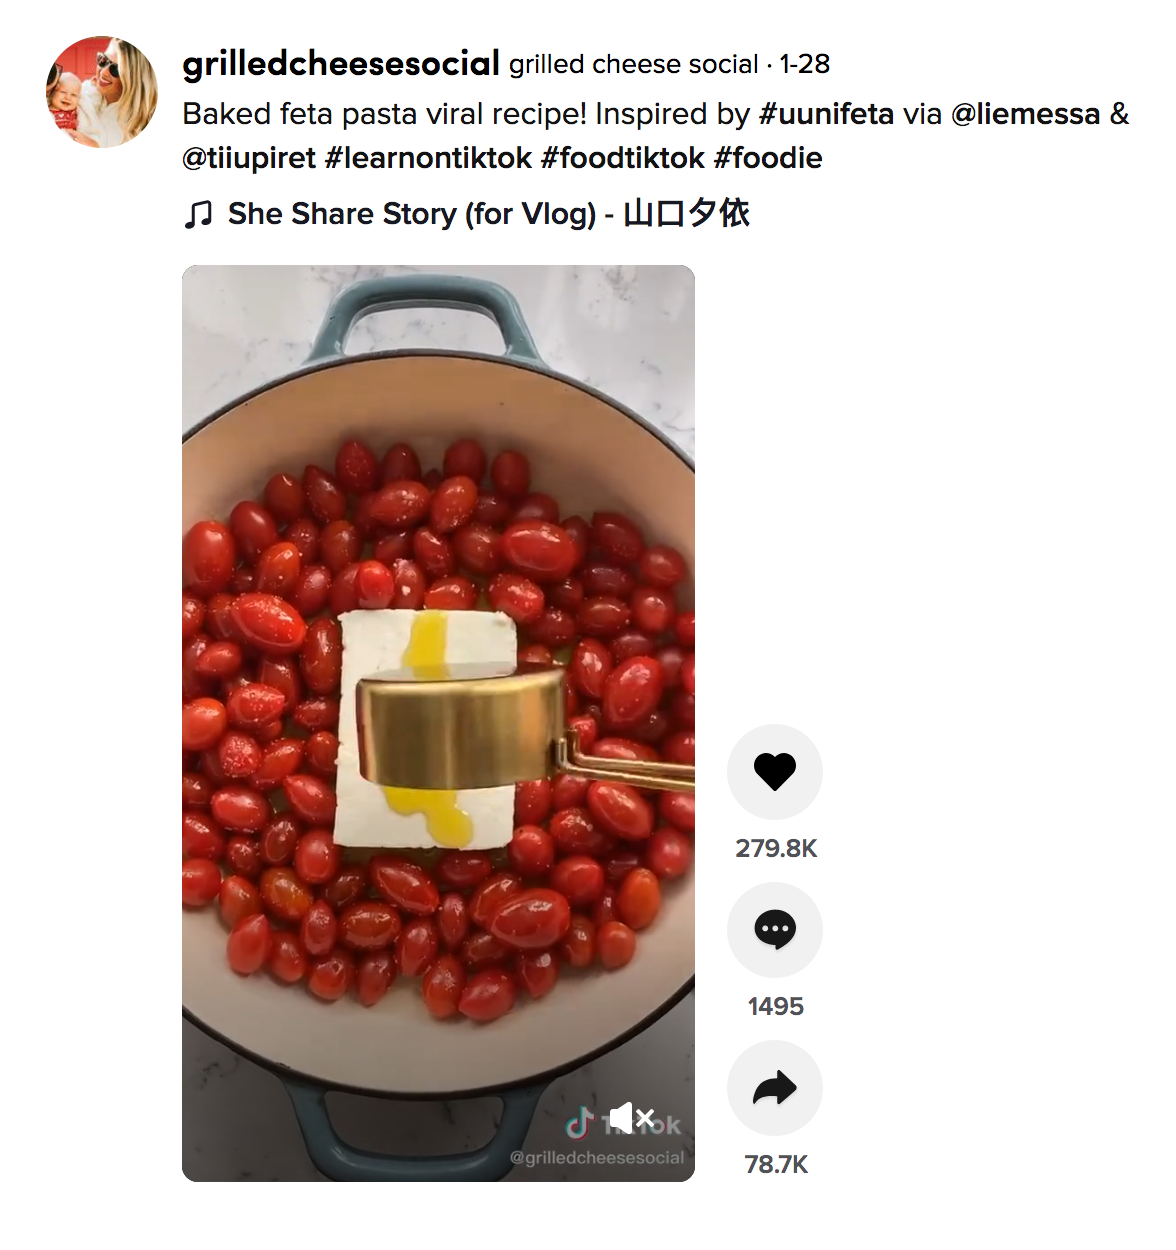
\includegraphics[height=0.8\textheight]{figures/tik_tok_feta_pasta}
\end{center}

\vfill

\url{https://www.tiktok.com/@grilledcheesesocial/video/6922946148760030469}

\note{
This recipe went viral.  What does this mean?  Here we want something more than just did it quickly become popular.  We want to trace person-to-person spread
}

\end{frame}
%%%%%%%%%%%%%%%%%%%%%
\begin{frame}

Similarities between the papers
\begin{itemize}
\item Both papers deal with a similar empirical phenomena and both struggle to figure out what is the \textbf{right question}
\pause
\item Both papers are in Pasteur's quadrant (motivated by use and seeking fundamental understanding)
\end{itemize}

\end{frame}
%%%%%%%%%%%%%%%%
\begin{frame}

\begin{center}
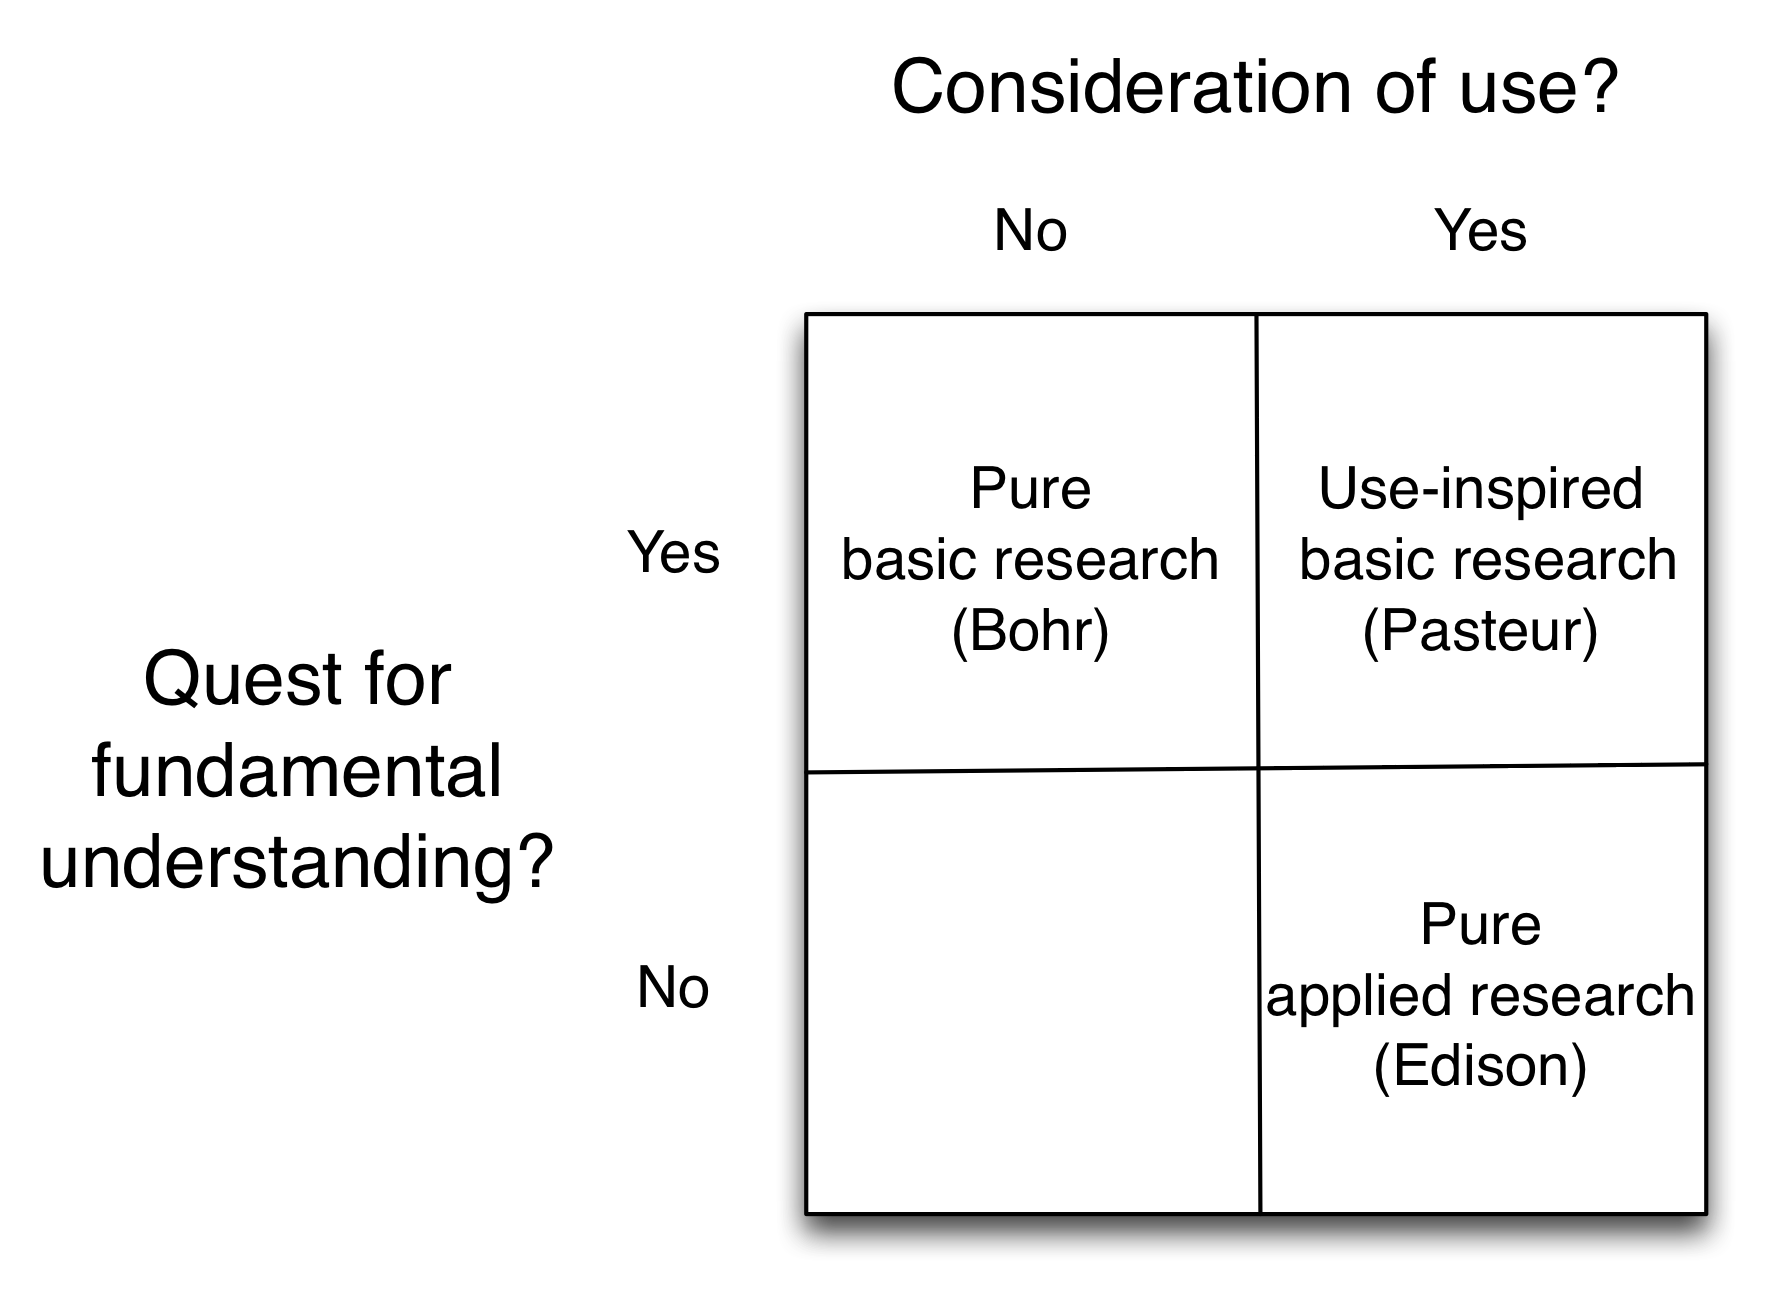
\includegraphics[width=0.7\textwidth]{figures/bitbybit4-17_pasteurs_quadrant}
\end{center}

\vfill
For more information, see Salganik (2018): \url{https://www.bitbybitbook.com/en/1st-ed/running-experiments/making/partner/}
\end{frame}
%%%%%%%%%%%%%%%%
\begin{frame}

\begin{itemize}
\item Both papers deal with a similar empirical phenomena and both struggle to figure out what is the \textbf{right question}
\item Both papers are in Pasteur's quadrant (motivated by use and seeking fundamental understanding)
\item Both papers include small and big cascades offering a systematic approach
\pause
\item Both papers require data that was not possible until recently
\pause
\item The papers end up with different ways of approaching the problem: descriptive vs predictive
\end{itemize}

\note{

Both ask interesting questions and different questions

}

\end{frame}
%%%%%%%%%%%%%%%%
\begin{frame}

\begin{center}
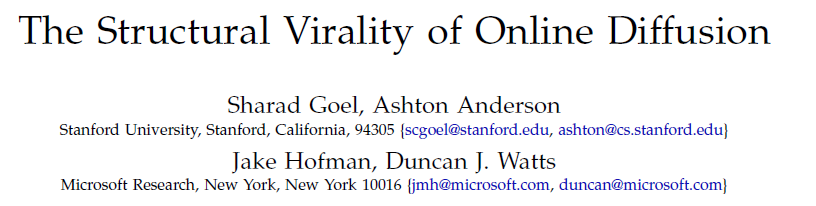
\includegraphics[width=0.9\textwidth]{figures/goel_structural_2016_title}
\end{center}

\end{frame}
%%%%%%%%%%%%%%%%%
\begin{frame}

What is virality?

\begin{center}
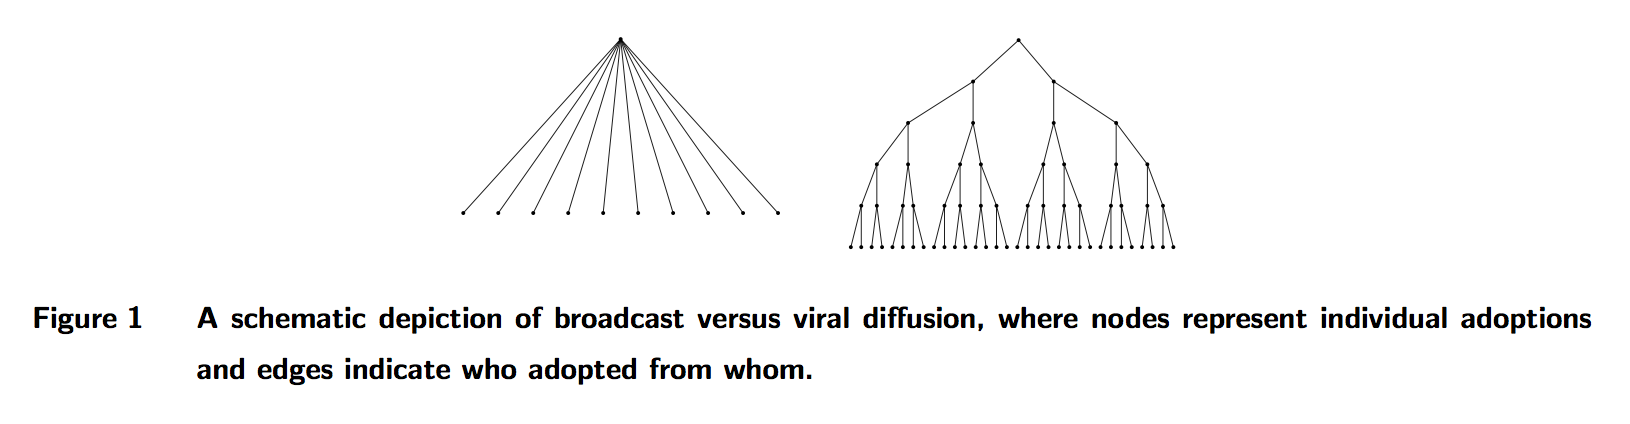
\includegraphics[width=1\textwidth]{figures/goel_structural_2016_fig1}
\end{center}

\end{frame}
%%%%%%%%%%%%%%%%%%%
\begin{frame}

Wiener index (from chemistry):

\begin{equation*}
\nu(T) = \frac{1}{n(n-1)}\sum_{i = 1}^n \sum_{j=1}^n d_{ij}
\end{equation*}
where $d_{i,j}$ is the length of the shortest path between $i$ and $j$ 
\vf
In other words, expected path length between two randomly chosen points

\note{
Walk through criteria that a measure should satisfy
Show problems with some existing metrics like depth
Propose this

People have adopted this metric
}

\end{frame}
%%%%%%%%%%%%%%%%%%%%%
\begin{frame}

\begin{columns}
\column{0.5\textwidth}

\begin{center}
\only<1>{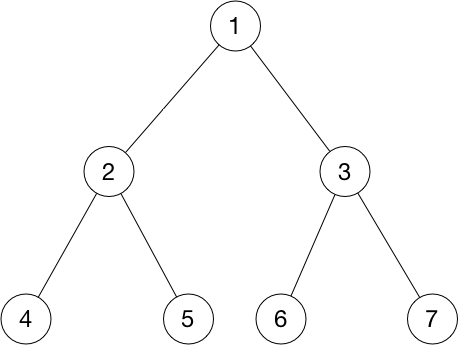
\includegraphics[width=0.6\textwidth]{figures/viral_tree}}%
\only<2>{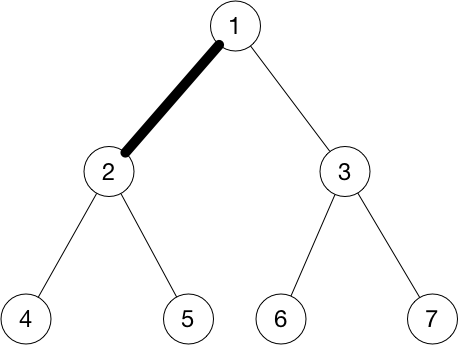
\includegraphics[width=0.6\textwidth]{figures/viral_tree_1-2}}%
\only<3>{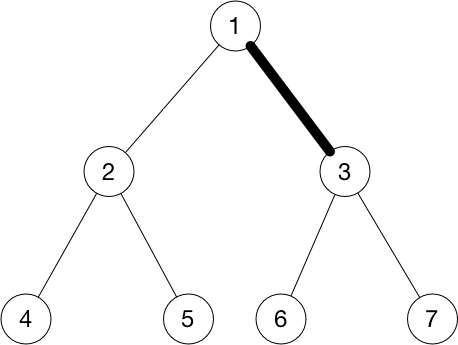
\includegraphics[width=0.6\textwidth]{figures/viral_tree_1-3}}%
\only<4>{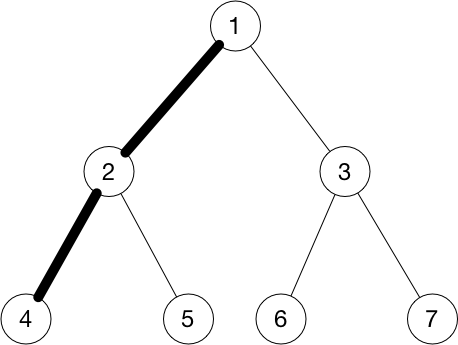
\includegraphics[width=0.6\textwidth]{figures/viral_tree_1-4}}%
\only<5>{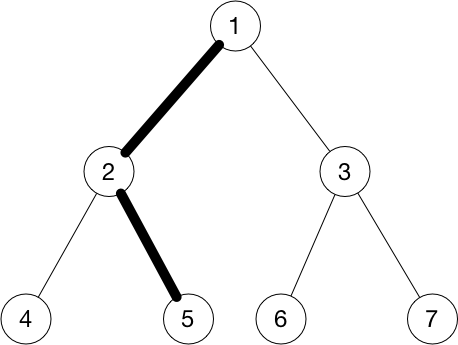
\includegraphics[width=0.6\textwidth]{figures/viral_tree_1-5}}%
\only<6>{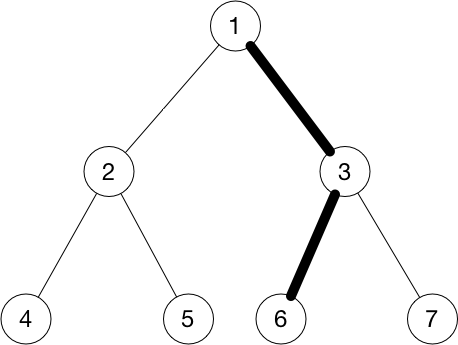
\includegraphics[width=0.6\textwidth]{figures/viral_tree_1-6}}%
\only<7>{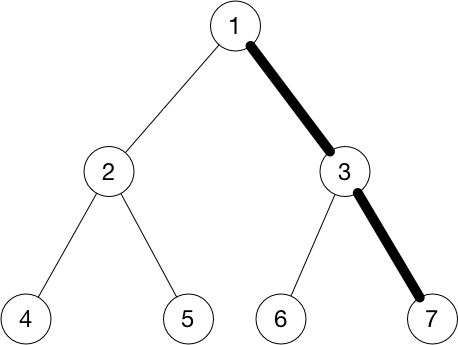
\includegraphics[width=0.6\textwidth]{figures/viral_tree_1-7}}%
\only<8->{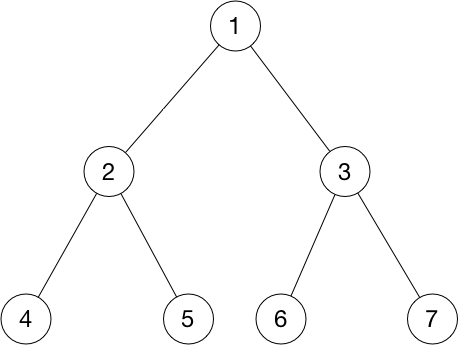
\includegraphics[width=0.6\textwidth]{figures/viral_tree}}%
\end{center}

\column{0.5\textwidth}

\begin{center}
\begin{tabular}{llllllll}
   & 1 & 2 & 3 & 4 & 5 & 6 & 7 \\
1 & 0 & \onslide<2->{1} & \onslide<3->{1} & \onslide<4->{2} & \onslide<5->{2} & \onslide<6->{2} & \onslide<7->{2} \\
2 & \onslide<8->{1 & 0 & 2 & 1 & 1 & 3 & 3} \\
3 & \onslide<9->{1 & 2 & 0 & 3 & 3 & 1 & 1} \\
4 & \onslide<10->{2 & 1 & 3 & 0 & 2 & 4 & 4} \\
5 & \onslide<11->{2 & 1 & 3 & 2 & 0 & 4 & 4} \\
6 & \onslide<12->{2 & 3 & 1 & 4 & 4 & 0 & 2} \\
7 & \onslide<13->{2 & 3 & 1 & 4 & 4 & 2 & 0} \\
\end{tabular}
\end{center}
\end{columns}

\onslide<14->{
\begin{equation*}
\nu(T) \approx 2.29 
\end{equation*}
}

\end{frame}
%%%%%%%%%%%%%%%%%%%%%
\begin{frame}

\begin{columns}
\column{0.5\textwidth}

\begin{center}
\only<1->{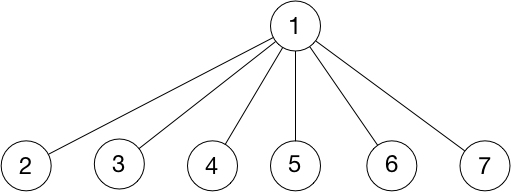
\includegraphics[width=0.6\textwidth]{figures/broadcast_tree}}%
\end{center}

\column{0.5\textwidth}

\begin{center}
\begin{tabular}{llllllll}
   & 1 & 2 & 3 & 4 & 5 & 6 & 7 \\
1 & 0 & \onslide<2->{1} & \onslide<3->{1} & \onslide<4->{1} & \onslide<5->{1} & \onslide<6->{1} & \onslide<7->{1} \\
2 & \onslide<8->{1 & 0 & 2 & 2 & 2 & 2 & 2} \\
3 & \onslide<9->{1 & 2 & 0 & 2 & 2 & 2 & 2} \\
4 & \onslide<10->{1 & 2 & 2 & 0 & 2 & 2 & 2} \\
5 & \onslide<10->{1 & 2 & 2 & 2 & 0 & 2 & 2} \\
6 & \onslide<10->{1 & 2 & 2 & 2 & 2 & 0 & 2} \\
7 & \onslide<10->{1 & 2 & 2 & 2 & 2 & 2 & 0} \\
\end{tabular}
\end{center}
\end{columns}

\vfill
\onslide<11->{
\begin{equation*}
\nu(T) \approx 1.71 
\end{equation*}
}

\end{frame}
%%%%%%%%%%%%%%%%%%%%%
\begin{frame}

\begin{columns}
\column{0.5\textwidth}

\begin{center}
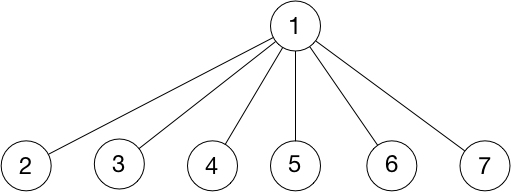
\includegraphics[width=0.6\textwidth]{figures/broadcast_tree}
$$\nu(T) \approx 1.71$$ 
\end{center}

\column{0.5\textwidth}
\begin{center}
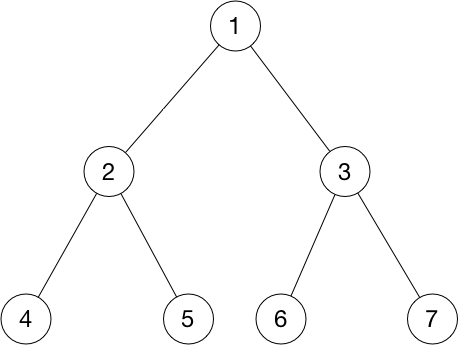
\includegraphics[width=0.6\textwidth]{figures/viral_tree}
$$\nu(T) \approx 2.29$$ 
\end{center}
\end{columns}

\end{frame}
%%%%%%%%%%%%%%%%%%%
\begin{frame}

\begin{center}
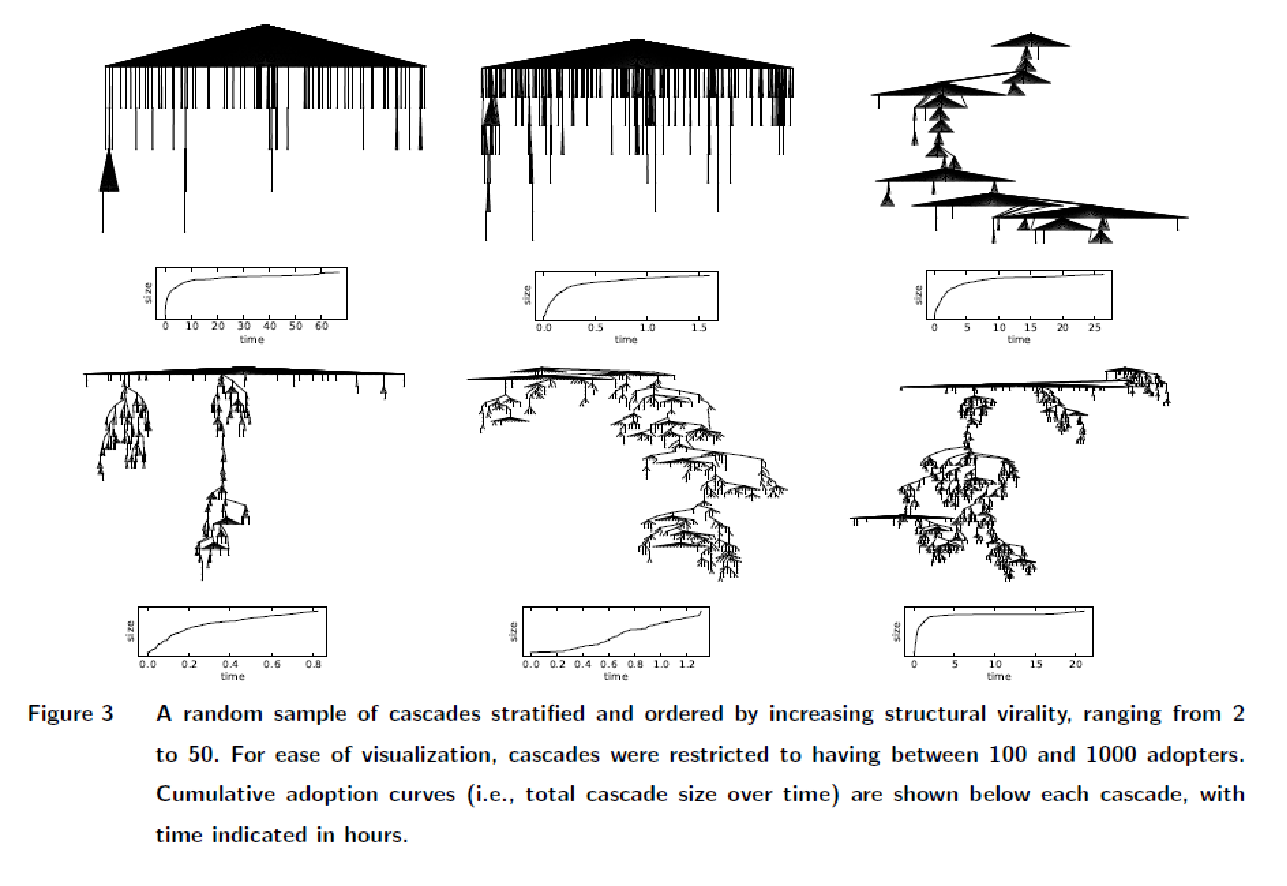
\includegraphics[width=0.9\textwidth]{figures/goel_structural_2016_fig3}
\end{center}

\end{frame}
%%%%%%%%%%%%%%%%%%%%%
\begin{frame}

describing outcomes vs describing generative process 

\end{frame}
%%%%%%%%%%%%%%%%%%
\begin{frame}

What do viral cascades look like?

\begin{itemize}
\item 622 million unique pieces of content (links) shared via Twitter
\item 1.2 billion adoptions (posting of content)
\item videos, images, news stories, and petitions
\end{itemize}

``Big data'' is needed because large cascades are very, very rare.

\end{frame}
%%%%%%%%%%%%%%%%%%
\begin{frame}

\begin{center}
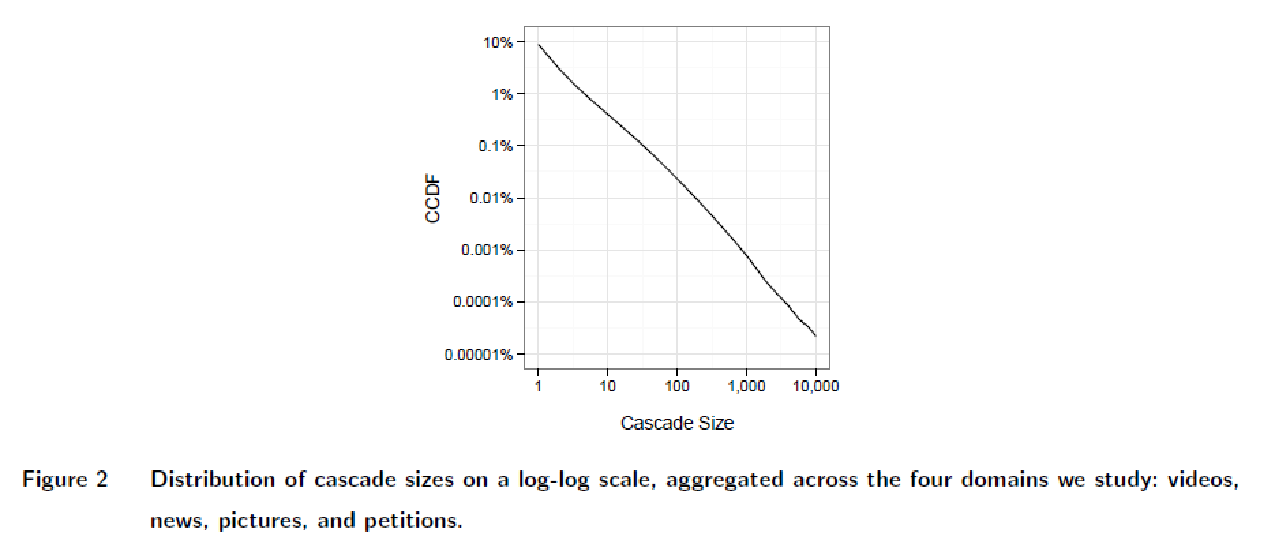
\includegraphics[width=0.8\textwidth]{figures/goel_structural_2016_fig2}
\end{center}

\begin{itemize}
\item Most things don't grow (99\% of adoptions are accounted for by the root node and the immediate followers of the root node) \pause
\item They focus on the cascades that include at least 100 nodes (1 in 4,000 events).
\end{itemize}

\end{frame}
%%%%%%%%%%%%%%%%%%
\begin{frame}

\begin{center}
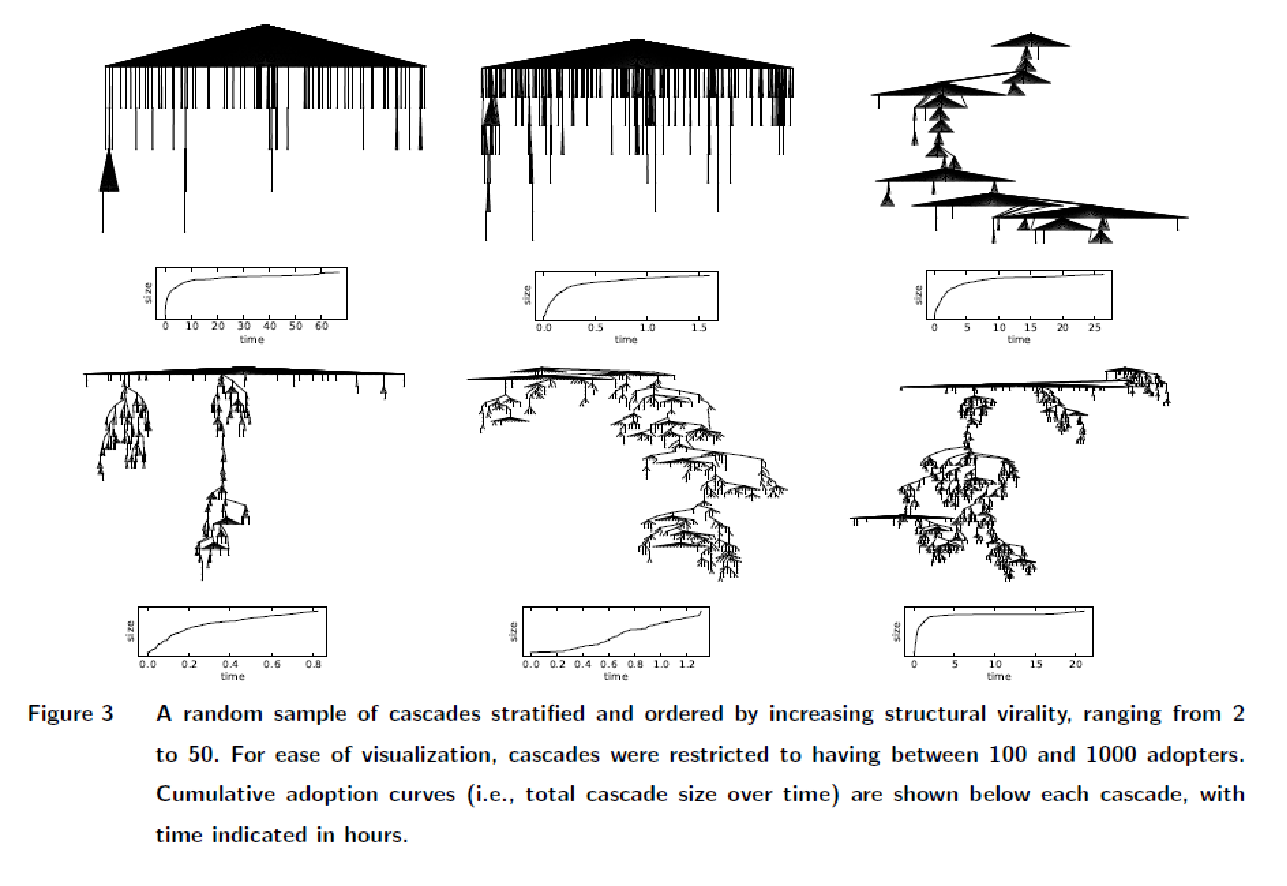
\includegraphics[width=0.7\textwidth]{figures/goel_structural_2016_fig3}
\end{center}

\begin{itemize}
\item Examples of different structural virality \pause
\item Structural virality captures something different from speed of adoption and diffusion curves
\end{itemize}

\end{frame}
%%%%%%%%%%%%%%%%%%%
\begin{frame}

\begin{center}
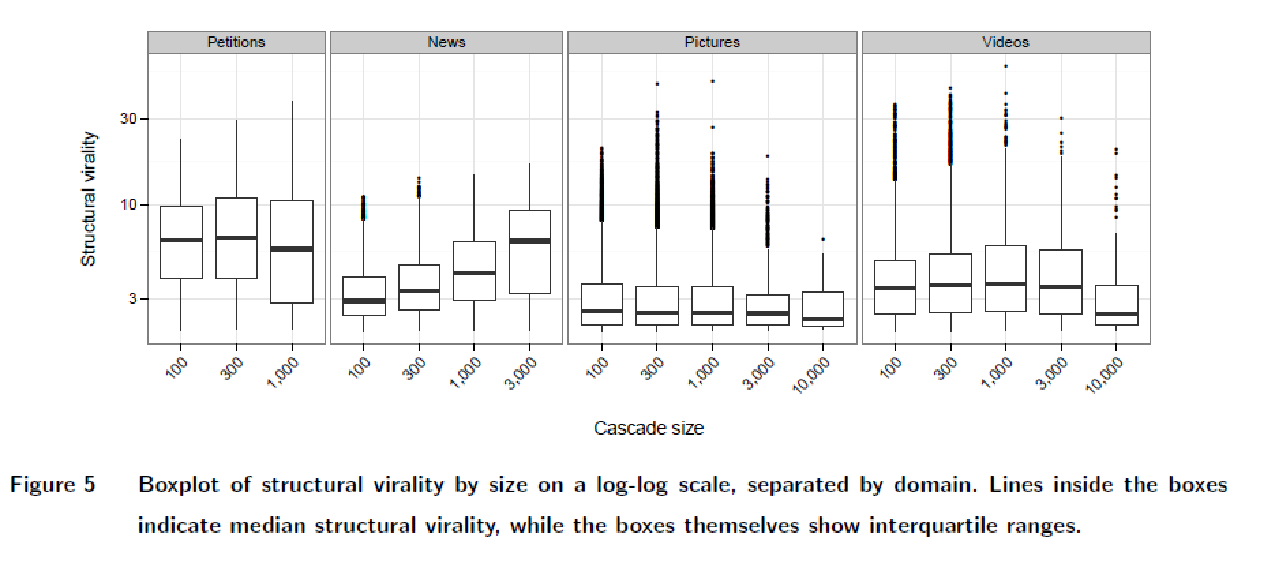
\includegraphics[width=\textwidth]{figures/goel_structural_2016_fig5}
\end{center}

Knowing the size of a cascades reveals little about structural virality.  This is true for all 4 types of content (but a bit less true for news).

\end{frame}
%%%%%%%%%%%%%%%%%%%
\begin{frame}

What combination of spreading process and network structure is consistent with these results?

\pause

SIR model on network with power law degree distribution

\end{frame}
%%%%%%%%%%%%%%%%%%%%
\begin{frame}

How might the ideas in this paper be used?
\vfill

\textcolor{blue}{\url{https://www.youtube.com/watch?v=wSwOszoHuoI}}

\end{frame}
%%%%%%%%%%%%%%%%%%%%%
\begin{frame}

Now we have a sense of what cascades can look like, but can they be predicted?

\end{frame}
%%%%%%%%%%%%%%%%%%%%%

\end{document}
